\documentclass[a4paper, 12pt]{article}%тип документа

%Русский язык
\usepackage[T2A]{fontenc} %кодировка
\usepackage[utf8]{inputenc} %кодировка исходного кода
\usepackage[english,russian]{babel} %локализация и переносы

%отступы 
\usepackage[left=2cm,right=2cm,top=2cm,bottom=3cm,bindingoffset=0cm]{geometry}

%Вставка картинок
\usepackage{graphicx}
\graphicspath{}
\DeclareGraphicsExtensions{.pdf,.png,.jpg, .jpeg}

%Таблицы
\usepackage[table,xcdraw]{xcolor}
\usepackage{booktabs}

%Графики
\usepackage{pgfplots}
\pgfplotsset{compat=1.9}

%Математика
\usepackage{amsmath, amsfonts, amssymb, amsthm, mathtools}

%Заголовок
\author{Подлесный Артём \\ группа 827}
\title{Работа 1.2.3 \\ Определение моментов инерции твердых тел с помощью трифилярного подвеса}

\begin{document}
\maketitle
\paragraph{Цель работы:}
измерение момента инерции ряда тел и сравнение результатов с расчетами по теоретическим формулами; проверка аддитивности моментов инерции и справедливости формулы Гьюгенса-Штейнера.
\paragraph{Оборудование:}
трифилярный подвес, секундормер, счетчик числа колебаний, набор тел, момент инерции которых надлежит измерить (диск, стержень, полый цилиндр и другие).
\section{Отчёт о работе}
\subsection{Общая теория}
Момент инерции твердого тела определяется по формуле
\begin{equation}
I=\int r^2dm.
\end{equation}
Для однородных твердых тел известной плотности при заданных размерах и достаточно простой форме момент инерции можно вычислить. Для неоднородных тел и тел сложной формы момент инерции можно определить экспериментально. Удобно использовать устройство, называемое трифилярным подвесом.

\begin{figure}[h!]
\center{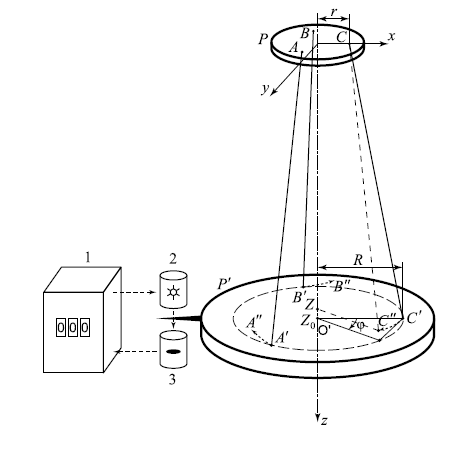
\includegraphics[scale=0.7]{trif.png}}
\caption{Трифилярный подвес.}
\end{figure}

Платформа снабжена рычагом, с помощью которого можно раскручивать верхний диск, который, в свою очередь, раскручивает нижний, не сообщая ему лишних колебаний в вертикальной плоскости. Количество колебаний считывается электронным счетчиком. Если пренебречь потерями энергии на трение, то ЗСЭ можно записать следующим образом:
\begin{equation}
\frac{I\dot{\varphi^2}}{2}+mg(z_0-z)=E
\end{equation}
Если $L$ -- длина нити, а угол $\varphi$ -- угол поворота, то т.к. при малых углах поворота $\cos{\varphi}\approx 1-\varphi^2/2$, получаем
\begin{equation}
z^2=L^2-R^2-r^2+2Rr\cos{\varphi}=z^2_0-2Rr(1-\cos{\varphi})\approx z^2_0-Rr\varphi^2.
\end{equation}
Извлекая отсюда квадратный корень и учитывая малость угла, имеем 
\begin{equation}
z\approx\sqrt{z^2_0-Rr\varphi^2}\approx z_0-\dfrac{Rr\varphi^2}{2z_0}.
\end{equation}
Подставляя это значение в (2) и дифференциируя его по времени, получаем
\begin{equation}
I\ddot{\varphi}+mg\frac{Rr}{z_0}\varphi=0.
\end{equation}
Решением этого уравнения будет
\begin{equation}
\varphi=\varphi_0\sin{\sqrt{\dfrac{mgRr}{Iz_0}}t+\theta}.
\end{equation}
Период крутильных колебаний нашей системы равен 
\begin{equation}
T=2\pi\sqrt{\dfrac{Iz_0}{mgRr}}.
\end{equation}
Отсюда находим формулу для определения момента инерции:
\begin{equation}
I=\dfrac{mgRrT^2}{4\pi^2z_0}.
\end{equation}
Удобно переписать это уравнение следующим образом:
\begin{equation}
I=kmT^2,
\end{equation}
где $k=\dfrac{gRr}{4\pi^2z_0}$ -- величина, постоянная для данной установки.
Таким образом, полученные формулы позволяют определить момент инерции платформы с телом и отдельно платформы по соответсвующим периодам крутильных колебаний. При выводе формул предполагалось, что малы необратимые потери энергии, связанные с трением, то есть мало затухание колебаний. О затухании колебаний можно судить, сравнивая время $\tau$ уменьшения амплитуды колебаний в пару раз с периодом колебаний $T$. Необратимыми потерями энергии можно пренебречь, если выполняется условие 
\begin{equation}
\tau\gg T.
\end{equation}
Это соотношение я проверил, добившись изменения амплитуды примерно в полтора раза за 260 секунд, при характерном периоде порядка 2 секунд, поэтому соотношение (10) выполняется достаточно хорошо.
\subsection{Экспериментальные данные}
\subsubsection{Параметры установки}
Измерим параметры установки:
\[R=115.4\pm0.5 \text{ мм},\]
\[r=30.5\pm0.1 \text{ мм},\]
\[L=216.5\pm0.5 \text{ cм},\]
\[z_0=216.3\pm0.7 \text{ см}.\]
Отсюда несложно получить параметр установки:
\[k=(4.040\pm0.044)\times 10^{-4}  m^2/c^2.\]
\subsubsection{Моменты инерции разных тел}
\paragraph{Момент инерции ненагруженной платформы}
оопределён, результаты представлены в следующей таблице:
\begin{table}[h]
\center{\begin{tabular}{|c|c|c|c|c|c|c|}
\hline
$N$ & $T_{10}$, с & $m_0$, г & $T$, c & $T_{\text{ср}}$, c & $I_0$, $\text{г}*\text{м}^2$ & $\sigma_I$, $\text{г}*\text{м}^2$ \\ \hline
10  & 44,16       &          & 4,416  &                    &            &                 \\ \cline{1-2} \cline{4-4}
11  & 48,55       &          & 4,414  &                    &            &                 \\ \cline{1-2} \cline{4-4}
11  & 48,58       & 993,5    & 4,416  & 4,416              & 7,83      & 0,15            \\ \cline{1-2} \cline{4-4}
10  & 44,23       &          & 4,423  &                    &            &                 \\ \cline{1-2} \cline{4-4}
10  & 44,1        &          & 4,410  &                    &            &                 \\ \hline
\end{tabular}}
\end{table}

Из этой таблицы, помимо всего прочего, можно выделить погрешность в срабатывании счетчика:
\[\sigma=4,219\times10^{-3} \text{ c}.\]
\paragraph{Моменты инерции ряда других тел. Аддитивность.}


Ниже представлена таблица для определения моментов инерции ряда тел, фотографии которых показаны чуть ниже.

\begin{table}
\centering
\begin{tabular}{|l|l|l|l|l|l|l|l|l|} 
\hline
Фигуры & $N$ & $\tau$, c & $T$, c & $m$, г & $I_{sum}$, $\text{г}*\text{м}^2$ & $\sigma_{I_s}$, $\text{г}*\text{м}^2$ & $I$, $\text{г}*\text{м}^2$ & $\sigma_I$, $\text{г}*\text{м}^2$  \\ 
\hline
Ф1      & 50     & 212,7                       & 4,254     & 1975,2    & 14,44               & 0,19                                  & 6,62       & 0,21                                 \\ 
\hline
Ф2      & 50     & 197,8                       & 3,956     & 1574,1    & 9,95               & 0,13                                  & 2,13       & 0,07                                \\ 
\hline
Ф1+Ф2   & 50     & 200,8                       & 4,016     & 2555,8    & 16,65               & 0,22                                  & 8,83       & 0,28                                \\ 
\hline
Ф3      & 50     & 187,9                       & 3,758     & 2068,5    & 11,8               & 0,2                                 & 3,98       & 0,13                                \\
\hline
\end{tabular}
\end{table}

Здесь первый столбец моментов инерции - моменты вместе с подставкой, второй -- с вычетом её момента инерции. С учетом погрешностей сумма моментов инерции Ф1 и Ф2 равна моменту импульса этих двух тел вместе, что подтверждает аддитивность моментов инерции.

Теперь рассчитаем теоретически значение момента инерции каждого из тел. 
\\ \\ \\ \\ \\ \\ \\ \\ \\ \\ \\ \\ \\ \\ \\ \\ \\ \\ \\ \\
На рисунке представлены все необходимые линейные размеры для определения момента инерции. Опустим расчеты, и полученные моменты инерции равны: 
\[I_1=(6.54\pm0.17) \text{  г}\times\text{м}^2,\]
\[I_2=(2.15\pm0.05) \text{  г}\times\text{м}^2,\]
\[I_3=(3.9\pm0.1) \text{  г}\times\text{м}^2.\]
Таким образом, с учётом погрешности, моменты импульса этих трёх тел, определеные экспериментально, совпадают с теоретическими значениями.
\subsubsection{Масса диска}
Зависимость периода крутильных колебаний системы от расстояния $h$ от полудиска до оси симметрии (как показано на фото), представлена в таблице:

\begin{table}[h]
\center{\begin{tabular}{|c|c|c|c|c|c|}
\hline
$h$, мм & $h^2$, $\text{мм}^2$ & $N$ & $\tau$, с & $T$, c & $T^2$, $c^2$ \\ \hline
0       & 0                    & 30  & 91,5      & 3,050  & 9,303        \\ \hline
5       & 25                   & 20  & 61,2      & 3,060  & 9,364        \\ \hline
10      & 100                  & 21  & 64,7      & 3,081  & 9,492        \\ \hline
15      & 225                  & 20  & 62,5      & 3,125  & 9,766        \\ \hline
20      & 400                  & 20  & 63,2      & 3,160  & 9,986        \\ \hline
25      & 625                  & 20  & 64,4      & 3,220  & 10,368       \\ \hline
30      & 900                  & 23  & 78,9      & 3,430  & 11,768       \\ \hline
35      & 1225                 & 22  & 73,8      & 3,355  & 11,253       \\ \hline
40      & 1600                 & 21  & 72,4      & 3,448  & 11,886       \\ \hline
45      & 2025                 & 20  & 71,1      & 3,555  & 12,638       \\ \hline
50      & 2500                 & 20  & 72,9      & 3,645  & 13,286       \\ \hline
55      & 3025                 & 20  & 75        & 3,750  & 14,063       \\ \hline
\end{tabular}}
\end{table}

\begin{figure}[h!]
\center{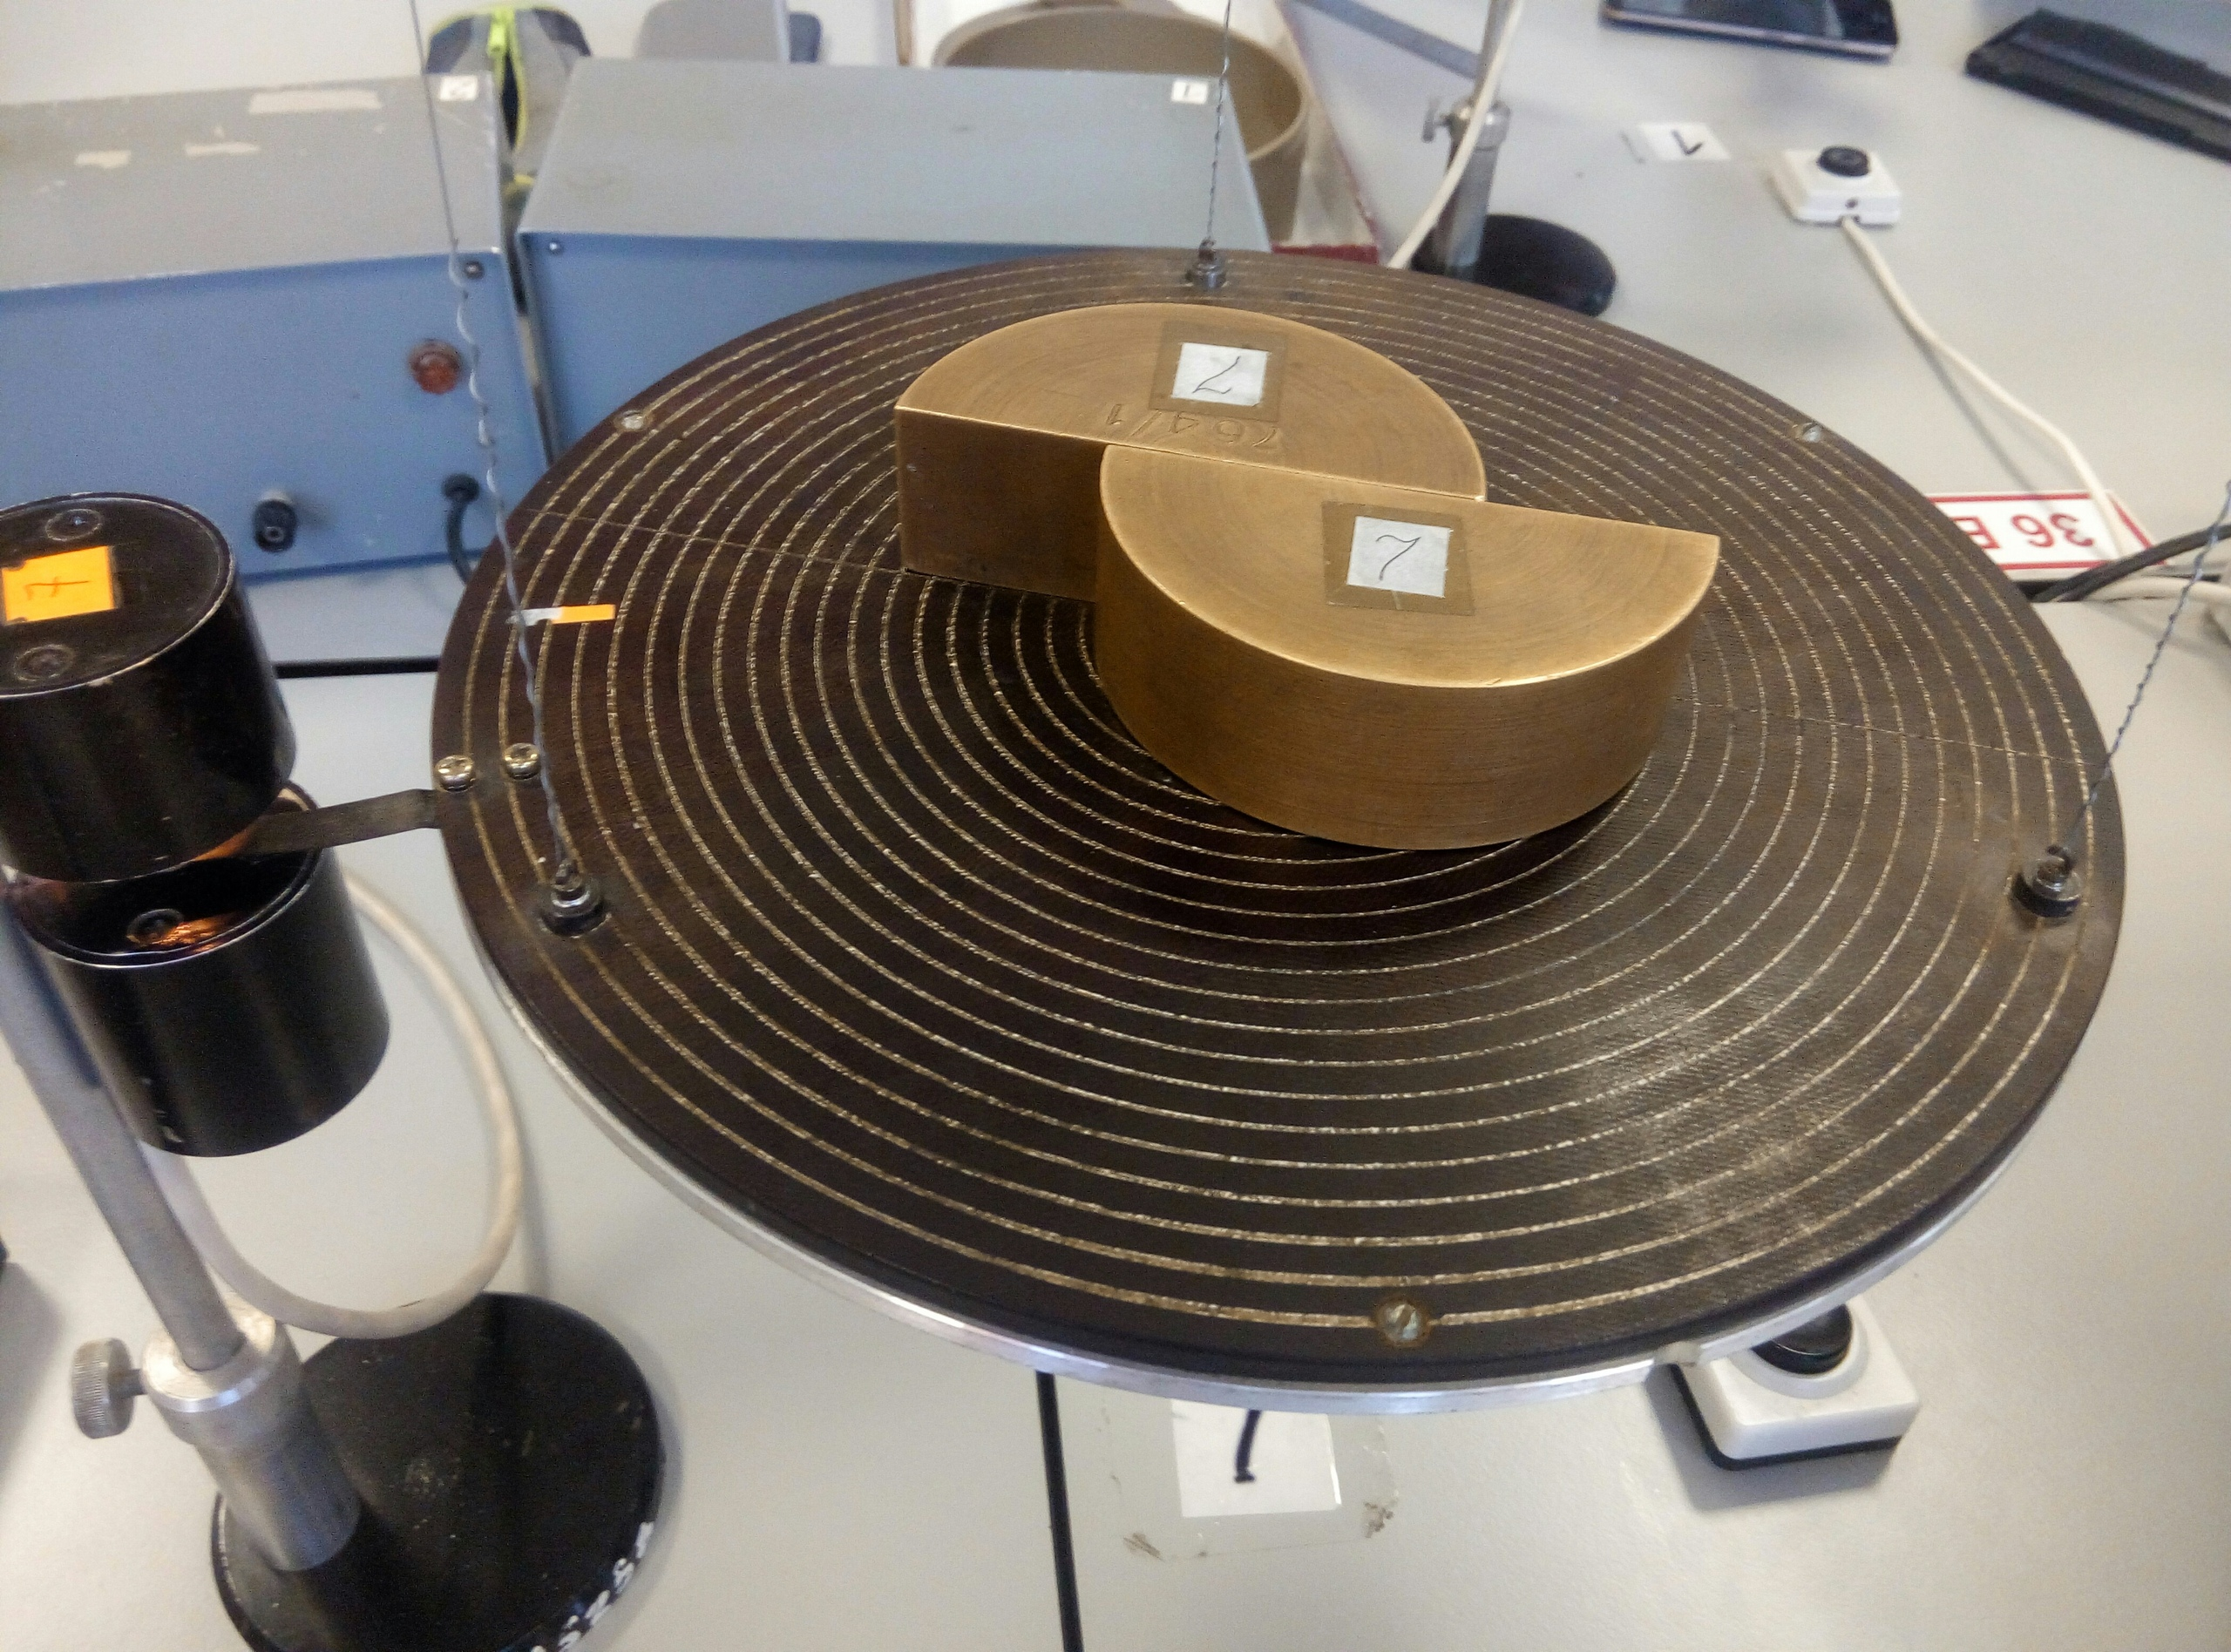
\includegraphics[scale=0.07]{f4.jpg}}
\caption{Смещение вдоль.}
\end{figure}

В силу теоремы Гьюгенса-Штейнера 
\[I=I_0+mh^2=k(m+m_0)T^2,\]
где $m$ масса двух половинок диска. Тогда график зависимости $T^2(h^2)$ должен оказаться линейным. Построим такой график.

\begin{figure}[h!]
\center{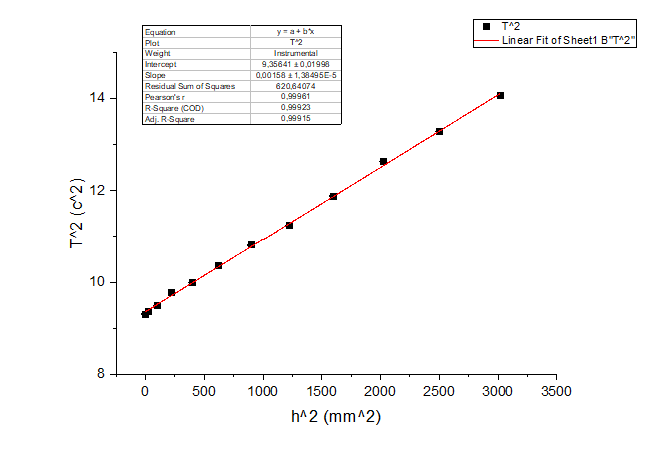
\includegraphics[scale=0.9]{gr1.png}}
\caption{Смещение вдоль.}
\end{figure}

Отсюда, зная, коэффициент наклона графика выражатся, как
\[t=\dfrac{m}{k(m+m_0)},\]
получаем, что масса диска равна:
\[m=m_0\dfrac{kt}{1-kt}=(1752\pm35)\text{ г}.\]
Непосредственно измеренная масса диска равна $1524.4\pm0.3$ г, из чего можно сделать вывод, что при проведении эксперимента была допущенна ошибка. В таком случае в экспериментальном определении момента инерции диска нет смысла.

\subsection{Поперечное смещение}
Снимем зависимость $T(h)$ при поперечном раздвигании полудисков (рис.4). Данные представены в таблице.

\begin{table}[h]
\center{\begin{tabular}{|c|c|c|c|c|c|}
\hline
$h$, мм & $h'$, $\text{c}^2$ & $N$ & $\tau$, с & $T$, c & $T^2-h'$, $c^2$ \\ \hline
0       & 0                  & 30  & 91,5      & 3,05   & 9,30            \\ \hline
5       & 0,0375             & 30  & 92,9      & 3,10   & 9,55            \\ \hline
10      & 0,15               & 20  & 63,2      & 3,16   & 9,84            \\ \hline
15      & 0,3375             & 21  & 68,1      & 3,24   & 10,18           \\ \hline
20      & 0,6                & 20  & 66,4      & 3,32   & 10,42           \\ \hline
25      & 0,9375             & 20  & 75,9      & 3,80   & 13,46           \\ \hline
30      & 1,35               & 22  & 77,4      & 3,52   & 11,03           \\ \hline
35      & 1,8375             & 21  & 76        & 3,62   & 11,26           \\ \hline
40      & 2,4                & 22  & 82,3      & 3,74   & 11,59           \\ \hline
45      & 3,0375             & 20  & 77,1      & 3,86   & 11,82           \\ \hline
\end{tabular}}
\end{table}

\begin{figure}[h!]
\center{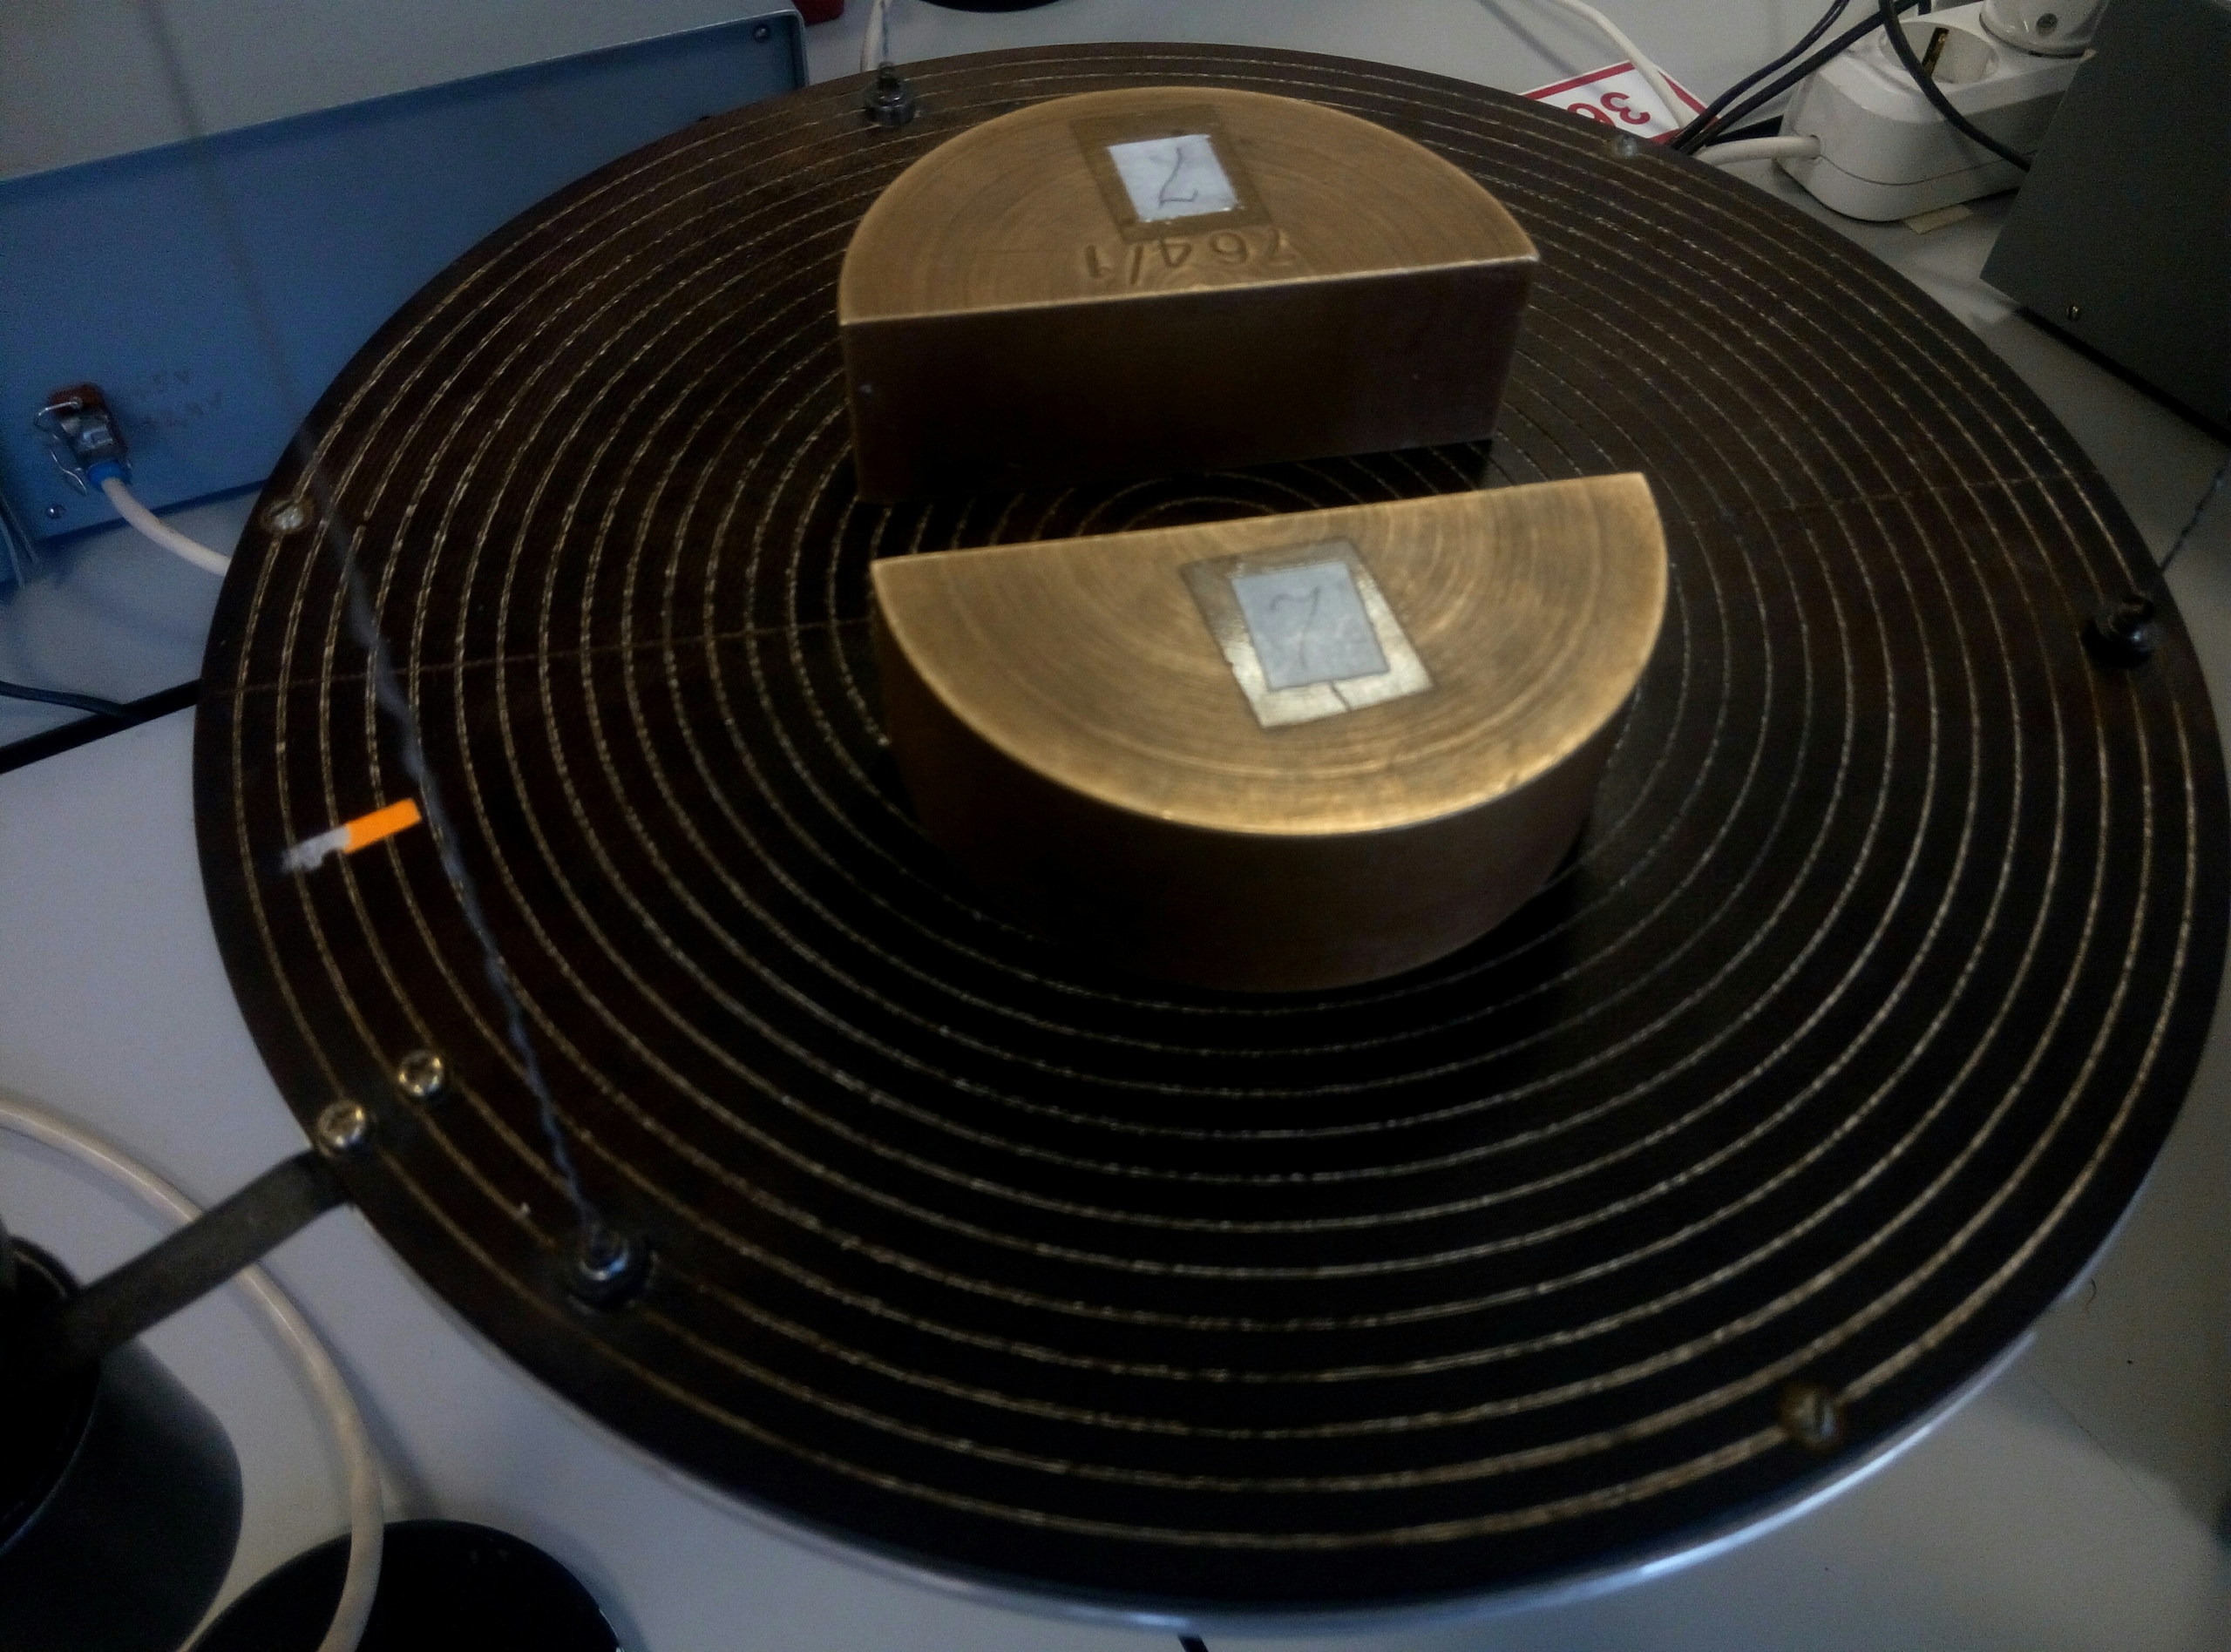
\includegraphics[scale=0.07]{f5.jpg}}
\caption{Смещение поперек.}
\end{figure}
 
Пусть $a$ -- расстояние от среза полудиска до его центра масс:
\\ \\ \\ \\ \\ \\ \\ \\ \\
Тогда по теореме Гьюгенса-Штейнера можно получить, что:
\[\alpha+m(h+a)^2=k(m+m_0)T^2.\]
Исходя из этого, если мы используем массу диска, измеренную на весах, то пусть приведенное расстояние будет -- $h'=h^2\frac{m}{k(m+m_0)}$, оно есть в таблице. Тогда получим такое уравнение:
\[T^2-h'=\dfrac{2ma}{k(m+m_0)}h+\dfrac{a^2m+\alpha}{k(m+m_0)},\]
из которого зависимость $(T^2-h')(h)$ будет линейной. Построим такой график.

\begin{figure}[h!]
\center{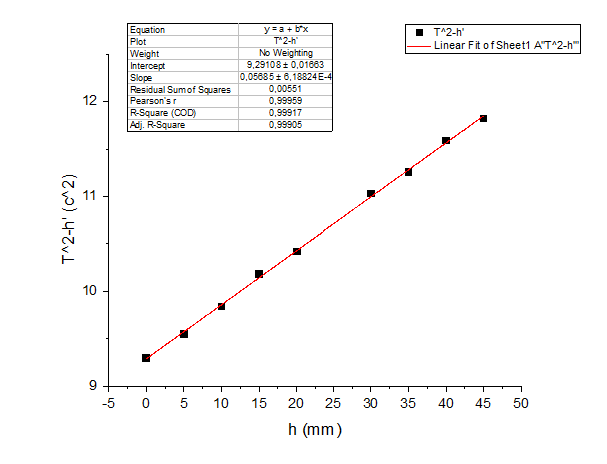
\includegraphics[scale=1.2]{gr2.png}}
\caption{Смещение поперек.}
\end{figure}

Так и получилось. Учитывая, что я брал точное значение массы, и всё получилось, этот эксперимент прошёл без ошибок. Из коэффициента наклона $t$ теперь можно вычислить $a$:
\[a=\dfrac{kt(m+m_0)}{2m}=(18.9\pm0.4)\text{ мм}.\]
Теоретическое значение для $a$ таково: $a=\frac{4R}{3\pi}$, из этого:
\[\pi=\frac{4R}{3a}=3.10\pm0.07.\]
Таким образом полученное значение числа Пи совпадает с реальным с учётом погрешности, поэтому можно считать, что эксперимент прошёл без ошибок, и является неплохим подтверждением теоремы Гьюгенса-Штейнера. 
\subsection{Масса диска при поперечном смещении}
Найдём с помощью этих экспериментальных данных массу диска. Используя ранее полученное соотношение, построим график зависимости $T^2((h+a)^2)$:

\begin{figure}[h!]
\center{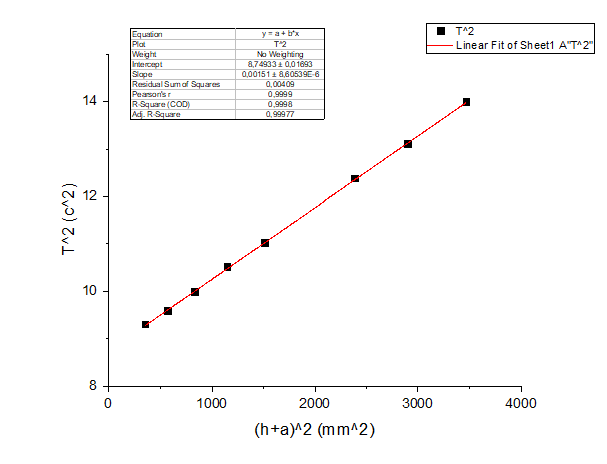
\includegraphics[scale=1.2]{gr3.png}}
\caption{Смещение поперек.}
\end{figure}

Отсюда масса диска равна:
\[m=(1554\pm27)\text{ г},\]
что уже совпадает с учетом погрешности со значением, измеренным на весах. Из этого можно померить и момент инерции диска: 
\[I_{\text{эксп}}=(5.84\pm0.17) \text{  г}\times\text{м}^2,\]
что согласуется  теоретическими расчетами.
\section{Вывод}
Были измерены моменты инерции ряда тел с хорошей точностью,была произведена проверка справедливости аддитивности моментов инерции и теоремы Гьюгенса-Штерна. Один эксперимент прошёл с ошибкой, которая скорее всего связана с тем, что положение центра масс системы в этом эксперименте сбилось, так как характер зависимости соответствует теории, но получилось неправильное значение. Однако следующим экспериментом я смог найти необходимые экспериментальные значения, и показать то, что планировалось показать первым экспериментом.









\end{document}